\documentclass[border = 10pt]{standalone}
%% Preamble %%
\usepackage{tikz}
\usepackage{newpxtext,newpxmath}            % upright Greek

\renewcommand{\familydefault}{\sfdefault}   % sans sarif
\usepackage{mathastext}                     % common look for text and maths

\usetikzlibrary{positioning, quotes, calc, arrows.meta, shapes, math}

\tikzset{
  every edge quotes/.style = {fill = white},
  > = {Stealth[length = 1.5mm]},       % Stealth arrowheads
  shorten > = 1pt,                     % Both ends of the arrows (ie, variances and covariances)       
  shorten < = 1pt,                     %    end 1pt short of the node
  manifest/.style = {draw, inner sep = 3pt, align = center, 
    minimum width = 1cm, minimum height = 0.85cm},
  latent/.style = {manifest, ellipse},
  residual/.style n args = {3}{inner sep = #1, minimum size = #2, #3},   % #3   draw
  residual/.default = {0}{0}{},                                
  constant/.style = {draw, inner sep = 1pt, minimum size = 5mm,
    regular polygon, regular polygon sides = 3},
  regression/.style = {->, shorten < = 0pt, inner sep = 1.5pt},
  covariance/.style n args = {3}{<->, inner sep = 1.5pt, bend #1 = #2, looseness = #3},
                        % #1  bend "right" or "left"; #2  bend angle; #3  looseness
  variance/.style n args = {3}{covariance = {#1}{#2}{#3}, inner sep = 0.5pt},
  interaction/.style = {-{Stealth[sep = 1pt, length = 1.5mm] . Circle[length = 4pt]},
    shorten > = -2pt},
  group/.style = {inner sep = 2pt, align = center, minimum width = 15mm, minimum height = 5mm}
}


\def \anglec {110, 90, 70}         % angles for intercepts leaving constant

\begin{document}
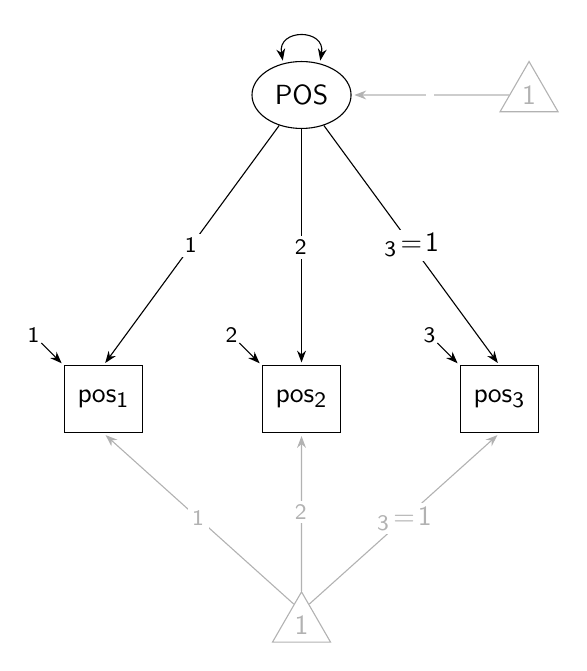
\begin{tikzpicture}

%% Indicators
\node [manifest] (pos1) {$pos_1$};
\node [manifest] (pos2) [right = 1.5cm of pos1] {$pos_2$};
\node [manifest] (pos3) [right = 1.5cm of pos2] {$pos_3$};

%% Latent and its variance
\node [latent] (POS) [above = 3cm of pos2] {$POS$};
\path [variance = {left}{100}{2.5}] (POS.120) edge ["$\upphi$" {above = 2pt}] (POS.60);

%% Consants and latent mean
\node [constant, black!30] (M1) [right = 2cm of POS] {1};
\node [constant, black!30] (M2) [below = 2cm of pos2] {1};
\path [regression, black!30] (M1) edge ["$\upkappa$"] (POS);

\foreach \j [count = \i] in \anglec { 
%% Loadings
\ifnum \i = 3 \def \lab {$\uplambda_3\!=\!1$} \else \def \lab {$\uplambda_\i$} \fi
\path [regression] (POS) edge ["\lab"] (pos\i.90);

%% Residuals
\node [residual] (e\i) [above left = 4mm of pos\i] {$\uptheta_\i$};
\path [regression] (e\i.south east) edge (pos\i.north west);

%% Intercepts
\ifnum \i = 3 \def \lab {$\uptau_3\!=\!1$} \else \def \lab {$\uptau_\i$} \fi
\path [regression, black!30] (M2.\j) edge ["\lab"] (pos\i.270);
}

\end{tikzpicture}
\end{document}
